\newthought{\textbf{Syarfani Akbar - 2020903430050 - TRKJ 3B}}

\newday{\textbf{1 - 2 Desember 2022} - instalasi Hadoop}
\begin{enumerate}
\item Kendala dan Solusi
pada praktikum ini tidak terjadi kendala.

\begin{figure}[!ht]
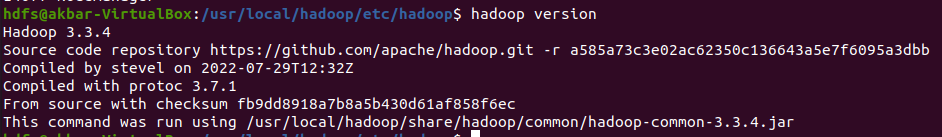
\includegraphics[width=.9\textwidth]{SyarfaniAkbar/install hadoop}
\caption{hasil hadoop version}
\label{gam:install hadoop}
\end{figure}

\item Kesimpulan
berhasil melakukan instalasi hadoop.
\end{enumerate}


\newpage
\newday{\textbf{8 Desember 2022} - WordCount Hadoop}
\begin{enumerate}
\item Kendala dan Solusi
pada praktikum ini tidak terjadi kendala.

\begin{figure}[!ht]
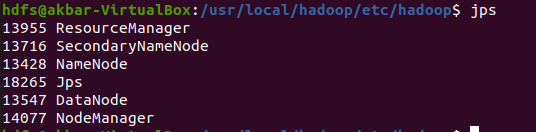
\includegraphics[width=.9\textwidth]{SyarfaniAkbar/cek hasil wordcount hadoop}
\caption{cek hasil wordcount hadoop menggunakan jps}
\label{gam:cek hasil wordcount hadoop}
\end{figure}

\begin{figure}[!ht]
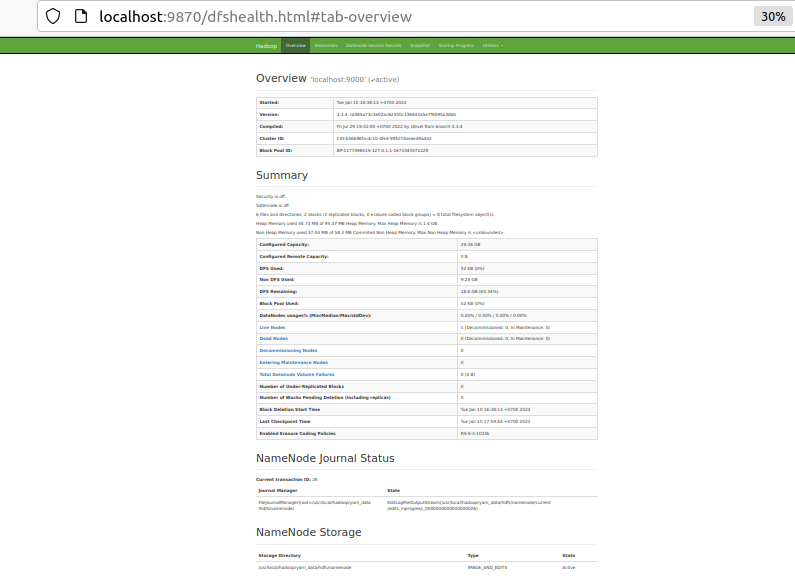
\includegraphics[width=.9\textwidth]{SyarfaniAkbar/hasil wordcount hadoop1}
\caption{hasil cek wordcount hadoop menggunakan website http://localhost:9870}
\label{gam:hasil wordcount hadoop1}
\end{figure}

\begin{figure}[!ht]
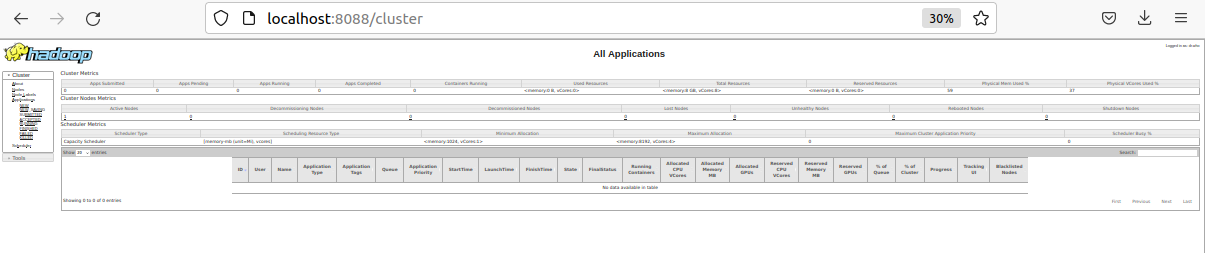
\includegraphics[width=.9\textwidth]{SyarfaniAkbar/hasil wordcount hadoop}
\caption{hasil cek wordcount hadoop menggunakan website http://localhost:8808}
\label{gam:hasil wordcount hadoop}
\end{figure}

\item Kesimpulan
berhasil melakukan konfigurasi wordcount hadoop.
\end{enumerate}

\newpage
\newday{\textbf{9 Desember 2022} - WordCount dengan Java}
\begin{enumerate}
\item Kendala dan Solusi
pada praktikum ini tidak terjadi kendala.

\begin{figure}[!ht]
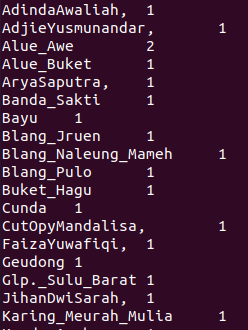
\includegraphics[width=.9\textwidth]{SyarfaniAkbar/hasil wordcount java}
\caption{hasil nama yang ada pada wordcount java}
\label{gam:hasil wordcount java}
\end{figure}

\newpage
\begin{figure}[!ht]
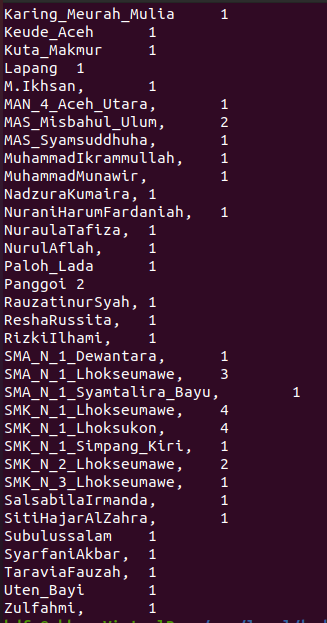
\includegraphics[width=.9\textwidth]{SyarfaniAkbar/cek hasil wordcount java}
\caption{lanjutan hasil nama yang ada pada wordcount java}
\label{gam:cek hasil wordcount java}
\end{figure}


\item Kesimpulan
berhasil melakukan konfigurasi wordcount java.
\end{enumerate}

